\documentclass[a4paper,landscape]{article} % Use A4 paper in landscape orientation
\usepackage{graphicx} % For including images
\usepackage{geometry} % For setting custom page margins
\usepackage{fancyhdr} % For customizing headers and footers
\usepackage[sfdefault]{roboto} % Set Roboto as the default sans-serif font
\usepackage{titlesec} % For customizing section titles
\usepackage{lastpage} % To reference the last page
\usepackage{hyperref} % For adding hyperlinks and bookmarks in the PDF

% Precise configuration of page margins
\geometry{
    a4paper,        % A4 paper format
    landscape,      % Landscape orientation
    top=0.9in,      % Top margin
    bottom=0.8in,   % Bottom margin
    left=0.5in,     % Left margin
    right=0.5in     % Right margin
}

% PDF bookmark settings
\hypersetup{
    bookmarks=true,         % Enable bookmarks in the PDF
    bookmarksopen=true,     % Open bookmarks by default
    bookmarksopenlevel=2,   % Level of bookmark expansion
    pdfpagemode=UseOutlines % Open PDF with bookmarks visible
}

% Define custom spacing and format for sections
\titleformat{\section}{\Large\bfseries}{\thesection.}{1em}{} % Format for sections
\titlespacing*{\section}{0pt}{-6pt}{0pt} % Adjust spacing around sections

% Custom headers and footers using fancyhdr
\pagestyle{fancy}
\fancyhf{} % Clear all header and footer fields

% Custom header settings
\fancyhead[L]{%
    \makebox[2cm][l]{From:} 2025-01-20 12:23:42\\ % Left header: Display "From" date
    \makebox[2cm][l]{To:} 2025-01-27 12:23:42      % Display "To" date
}
\fancyhead[C]{ % Centered header
    \huge\textbf{Flex Reversy 1}\\ % Main title
    \normalsize\textbf{Reversy Kiln - Overview} % Subtitle
}
\fancyhead[R]{ % Right header
    Page \thepage{} of \pageref{LastPage}\\ % Page number and total pages
    \small 1W range \textbar{} interval 3H % Display time range and interval
}

% Footer settings
\fancyfoot[L]{\small SET Sviluppo e Tecnologia\\} % Footer text on the left
\fancyfoot[C]{\small \\} % Footer text in the center
\fancyfoot[R]{\small Cimprogetti\\} % Footer text on the right

% Uncomment for alternate page numbering in the footer
%\fancyfoot[C]{\Large\thepage/\pageref{LastPage}} % Centered page number

\renewcommand{\headrulewidth}{0.4pt} % Thickness of the header line
% \renewcommand{\footrulewidth}{0.4pt} % Uncomment for footer line

\begin{document}
\setlength{\unitlength}{1pt}

\makebox[0pt][l]{\rule{0pt}{1pt}}
\section{Info}

\begin{picture}(0,0)(-20,-15)
\put(0,-85){
\includegraphics[width=240pt,height=68pt]{temp/images/panel_0001-0000.png}}
\put(240,-85){
\includegraphics[width=240pt,height=68pt]{temp/images/panel_0001-0008.png}}
\put(480,-85){
\includegraphics[width=240pt,height=68pt]{temp/images/panel_0001-0016.png}}
\put(0,-153){
\includegraphics[width=720pt,height=68pt]{temp/images/panel_0005-0000.png}}
\put(0,-204){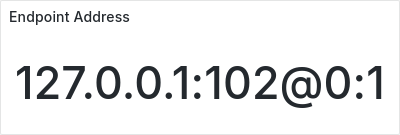
\includegraphics[width=150pt,height=51pt]{temp/images/panel_0009-0000.png}}
\put(150,-255){
\includegraphics[width=270pt,height=102pt]{temp/images/panel_0009-0005.png}}
\put(420,-204){
\includegraphics[width=150pt,height=51pt]{temp/images/panel_0009-0014.png}}
\put(570,-255){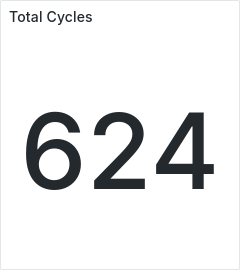
\includegraphics[width=90pt,height=102pt]{temp/images/panel_0009-0019.png}}
\put(660,-204){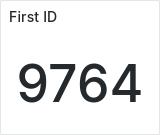
\includegraphics[width=60pt,height=51pt]{temp/images/panel_0009-0022.png}}
\put(0,-255){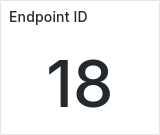
\includegraphics[width=60pt,height=51pt]{temp/images/panel_0012-0000.png}}
\put(60,-255){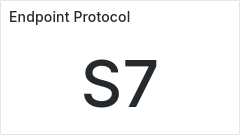
\includegraphics[width=90pt,height=51pt]{temp/images/panel_0012-0002.png}}
\put(420,-255){
\includegraphics[width=150pt,height=51pt]{temp/images/panel_0012-0014.png}}
\put(660,-255){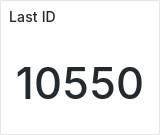
\includegraphics[width=60pt,height=51pt]{temp/images/panel_0012-0022.png}}
\put(0,-289){
\includegraphics[width=720pt,height=17pt]{temp/images/panel_0016-0000.png}}
\put(0,-340){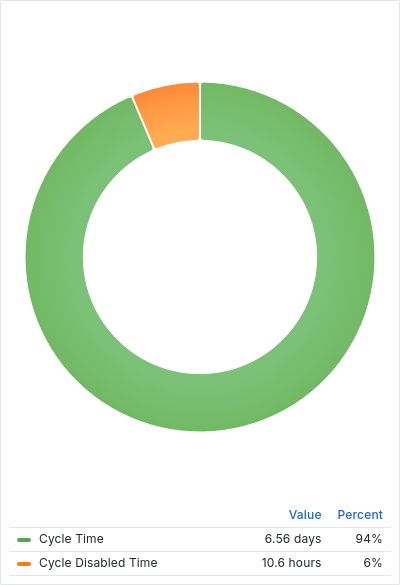
\includegraphics[width=720pt,height=17pt]{temp/images/panel_0019-0000.png}}
\end{picture}

\newpage

\makebox[0pt][l]{\rule{0pt}{1pt}}
\section{Table}

\begin{picture}(0,0)(-20,-15)
\put(0,-136){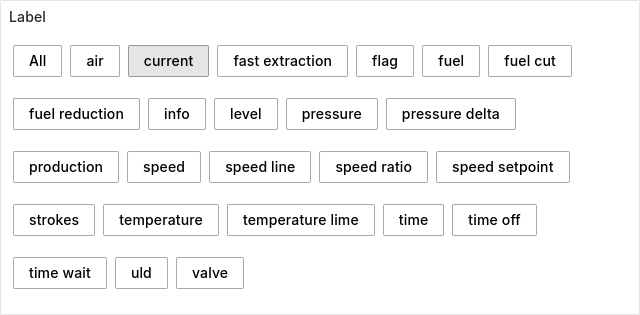
\includegraphics[width=240pt,height=119pt]{temp/images/panel_0025-0000.png}}
\put(240,-136){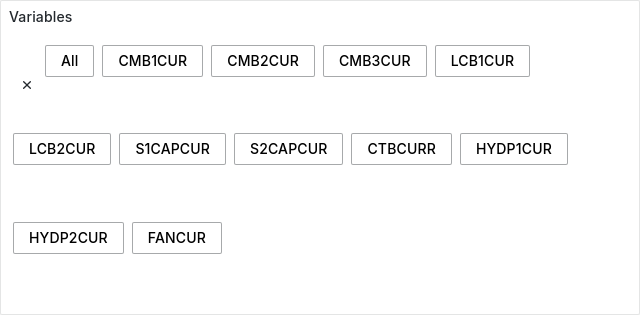
\includegraphics[width=240pt,height=119pt]{temp/images/panel_0025-0008.png}}
\put(480,-136){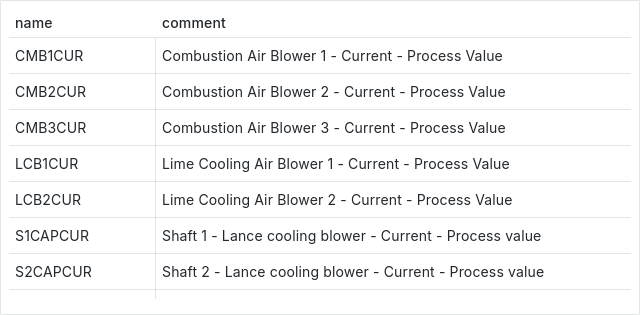
\includegraphics[width=240pt,height=119pt]{temp/images/panel_0025-0016.png}}
\put(0,-459){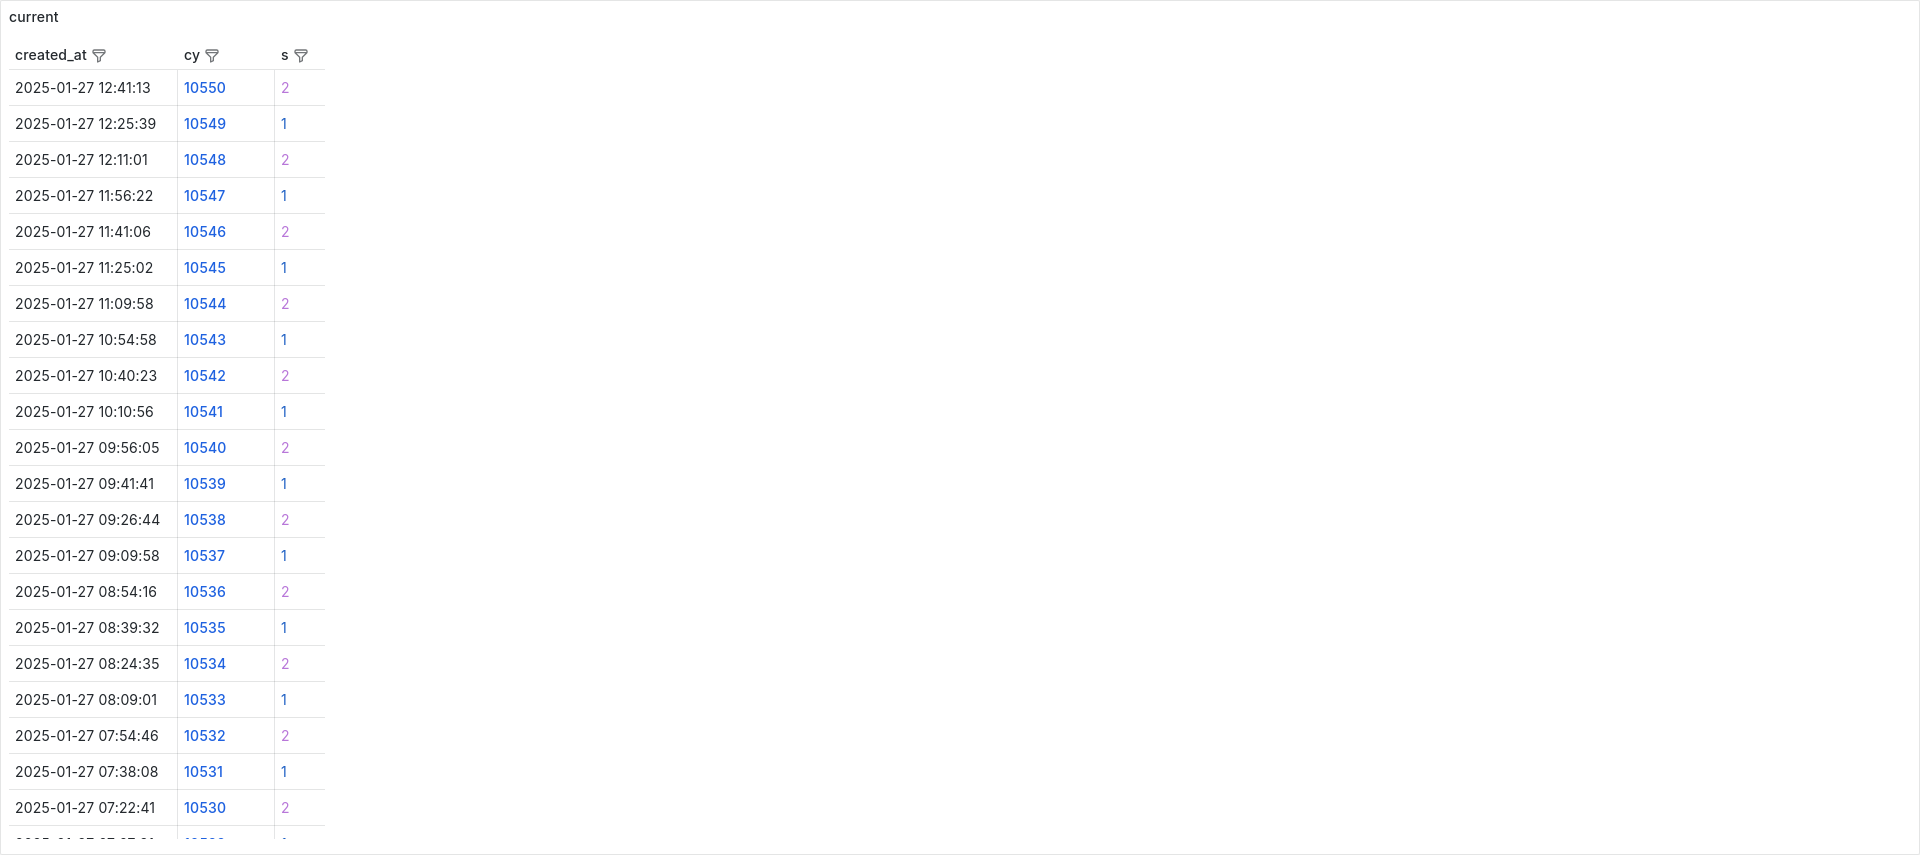
\includegraphics[width=720pt,height=323pt]{temp/images/panel_0032-0000.png}}
\end{picture}

\newpage

\begin{picture}(0,0)(-10,0)
\put(0,-255){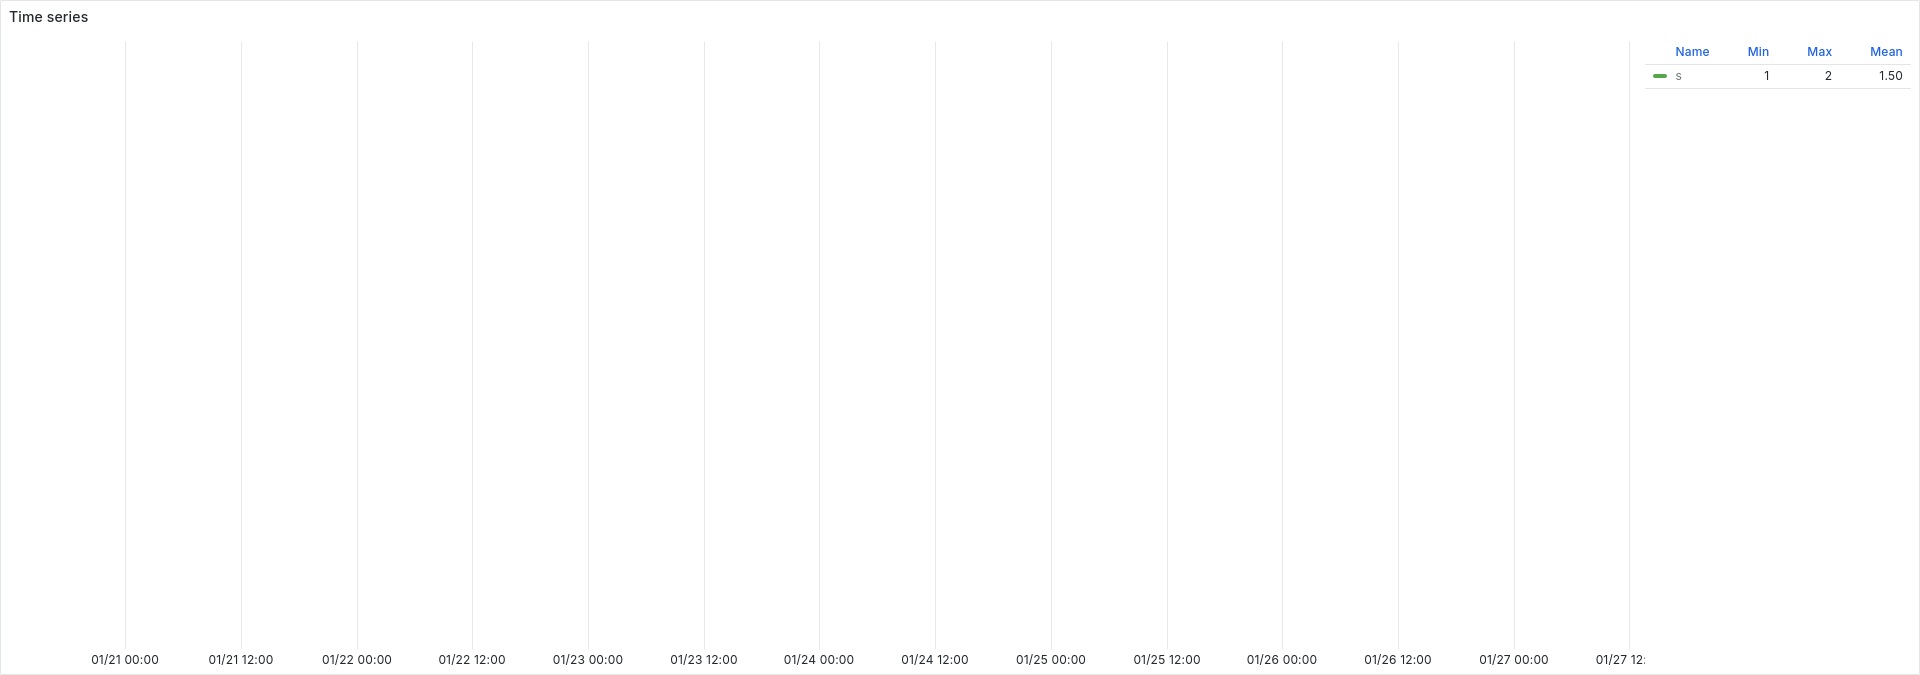
\includegraphics[width=720pt,height=255pt]{temp/images/panel_0051-0000.png}}
\end{picture}

\end{document}
 % Placeholder for the main content

